\chapter{Nozzle simulation and fluid mechanics primer}
\label{chap:Theory-CFD}
This chapter delves into the nozzle flow dynamics of a High-speed Orienting Momentum with Enhanced Reversibility (HOMER) nozzle, developed by Trancossi and Dumas \cite{trandum}. We begin with an understanding of the problem and the underlying principle, which is the Coanda effect. In Section \ref{goveq}, we elucidate the governing equations that mathematically define the fluid flow, as well as additional equations for turbulence modelling. Subsequently, we discuss various numerical approaches that discretize the governing equations. Additionally, the chapter provides insights into the simulation setup in Section \ref{setup}, encompassing meshing strategies, boundary condition specifications, and solver settings for the problem. 
\section{Jet deflection in the HOMER nozzle}  
The HOMER nozzle is designed to produce a controllable and selective deviation of a synthetic jet, generated by mixing two primitive jets. The jet is controlled solely by taking advantage of the Coanda effect and does not require any mechanical parts. The general structure of the nozzle is depicted in Figure \ref{fig:nozzle}. As we can see from the figure, the nozzle has two inlets fed by two impinging jets, followed by a convergence zone, or a septum, where mixing of the flows occurs. This generates a synthetic outflow jet, which can be controlled by modifying the momentums of the primitive jets. Next to the convergence zone is the outflow mouth, with curved walls connected to two convex Coanda surfaces on the top and bottom.
\begin{figure}[ht]
  \centering
  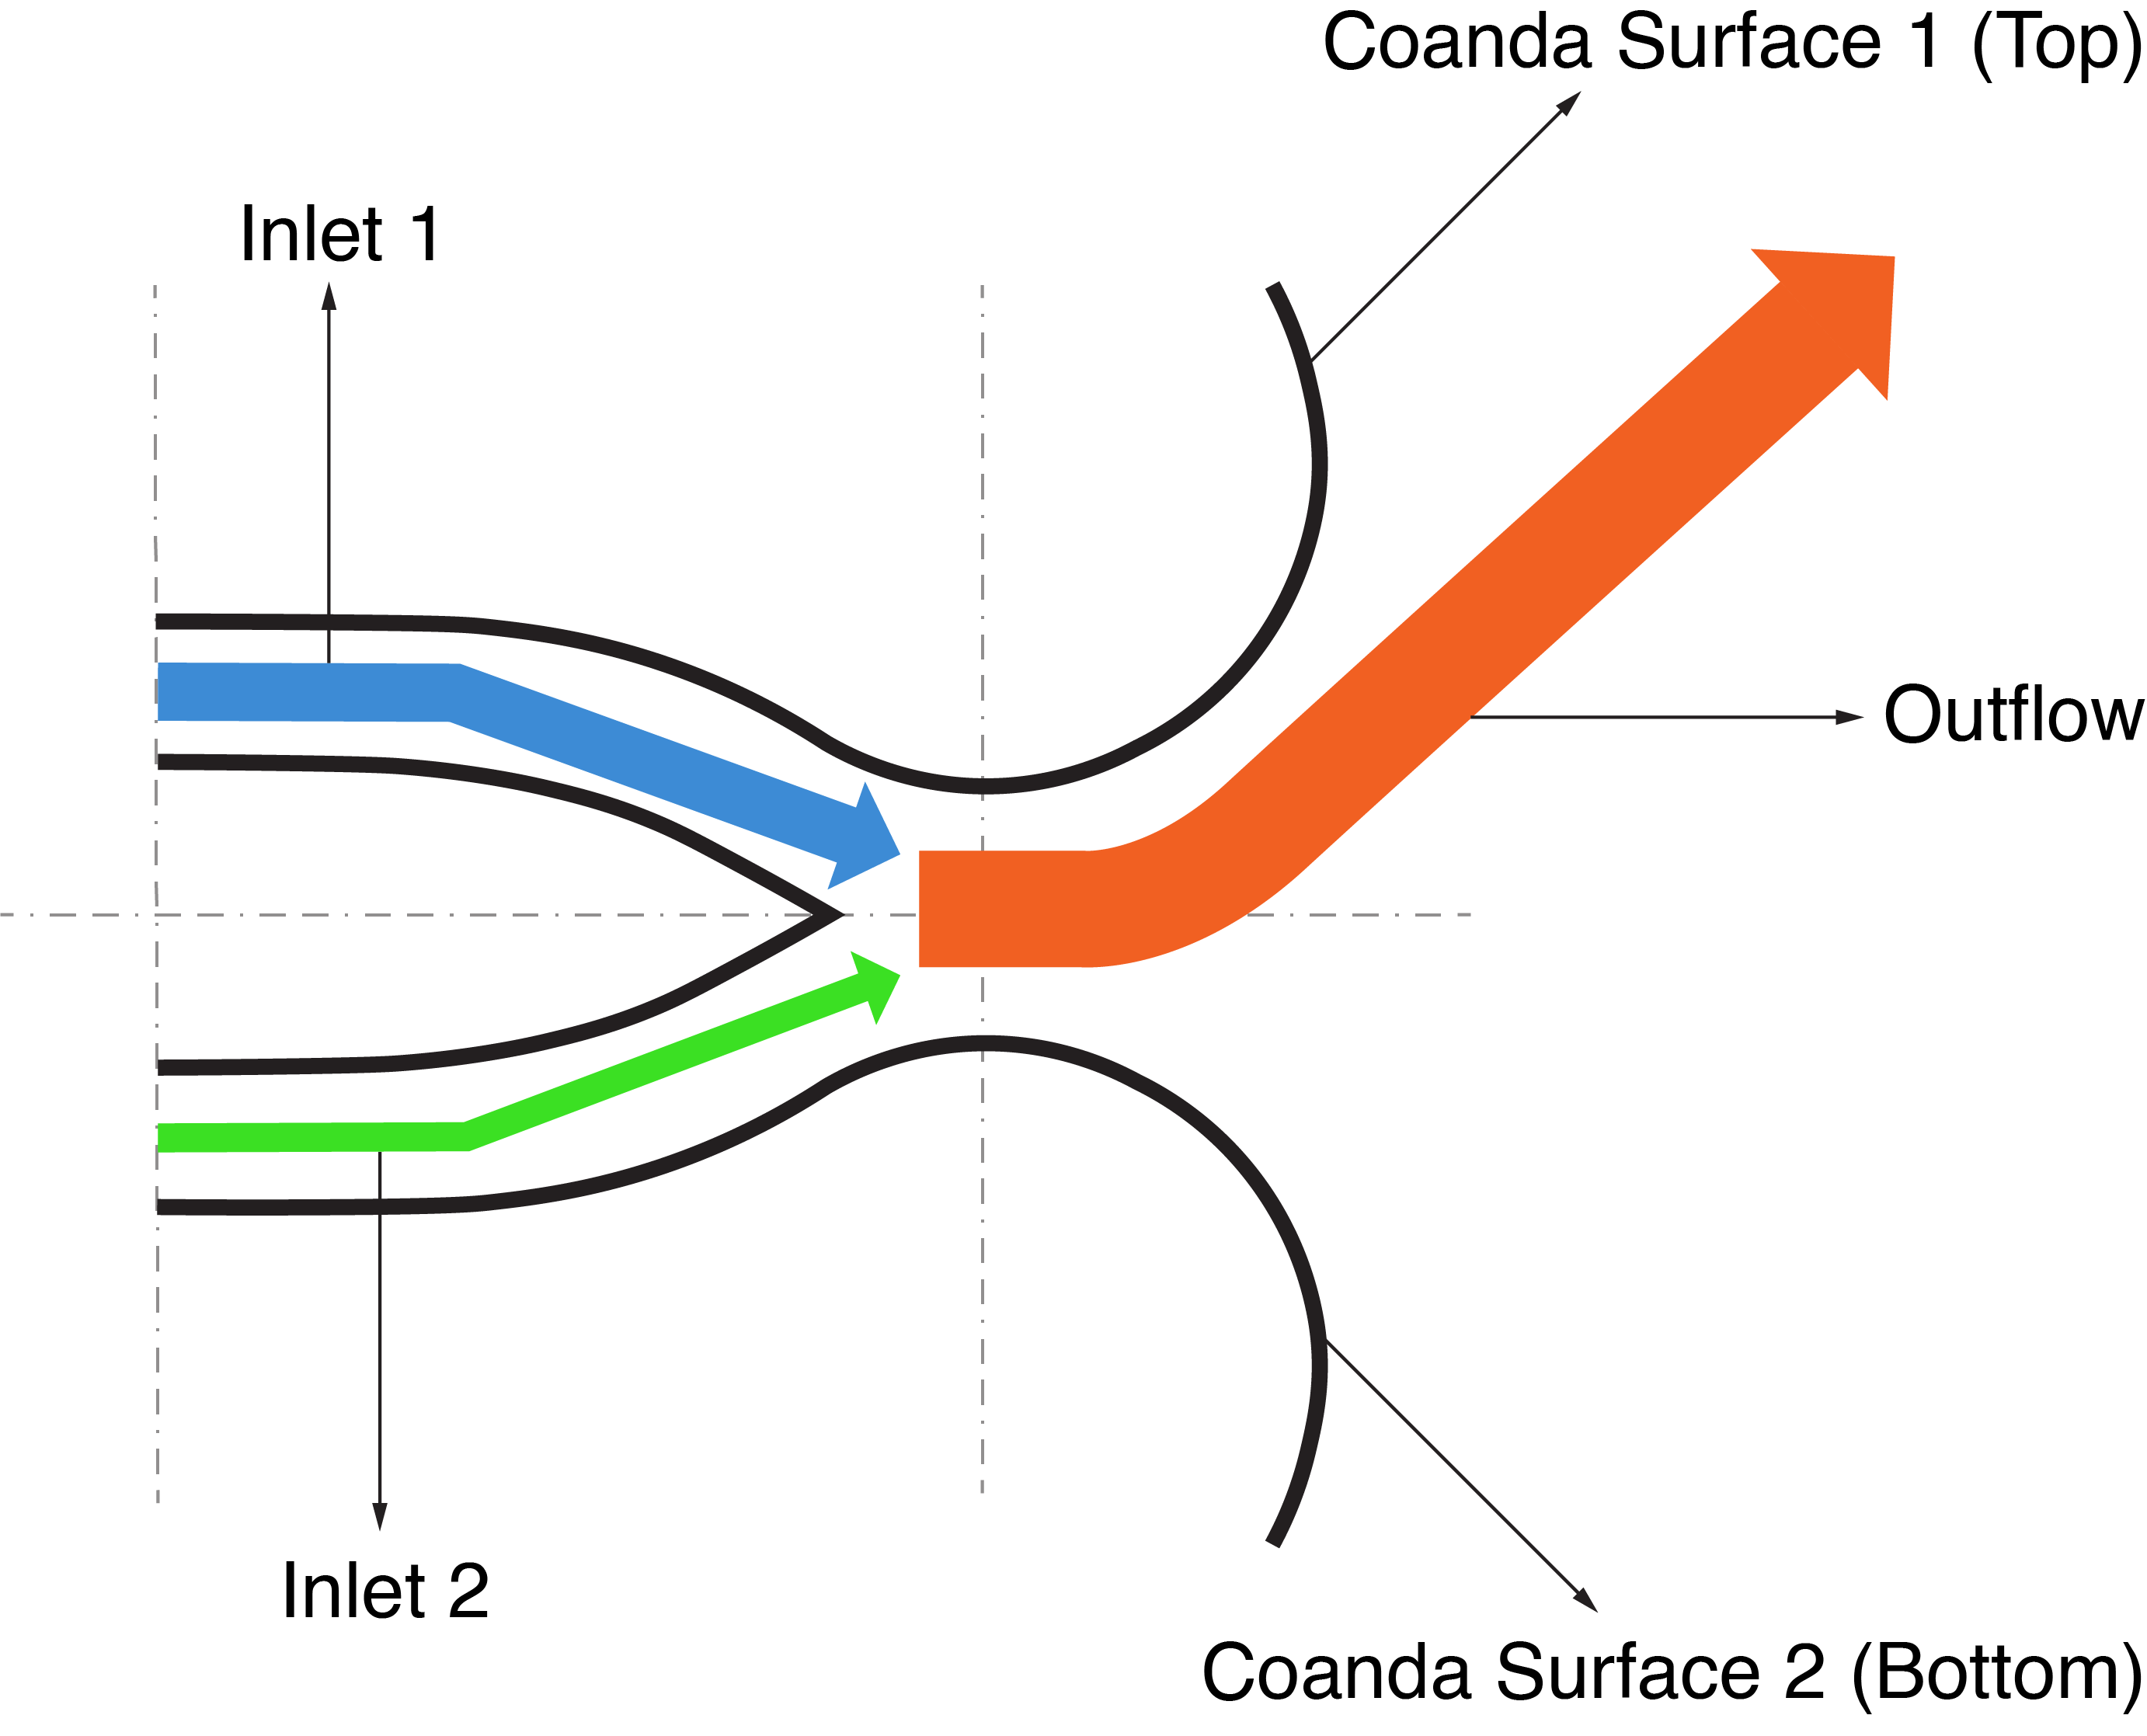
\includegraphics[width=8cm]{images/Theory-CFD/nozzle.png}
  \caption{Schematic overview of the HOMER nozzle design, highlighting the dual inlets and Coanda effect surfaces, adapted from Trancossi and Dumas \cite{trandum}}
  \label{fig:nozzle}
\end{figure}
The system requires a minimum operating condition of the primitive jets \cite{trandum} to ensure effective mixing. The impinging jets must have velocities high enough to generate a synthetic jet of Reynolds number greater than 5000 at the outlet mouth. To guarantee optimum operation, the Reynolds number at the outlet must exceed 10000. In the case of lower Reynolds numbers, the system's behavior is unpredictable. 
\subsection{Coanda effect}
Coanda effect is the tendency of a stream of fluid emerging from an orifice to follow an adjacent flat or curved surface and to entrain fluid from the surroundings so that a region of lower pressure develops. In simple terms, it is the tendency of a fluid to adhere to and stay attached to the walls of a convex surface, as demonstrated in Figure \ref{fig:Coanda}. Different fluid dynamic effects concur to create the Coanda effect, namely the boundary layer effect, the adhesion effect, and the attraction effect. Newman \cite{newman} has demonstrated that Coanda adhesion to a curved surface is dependent on the equilibrium of forces applied on the fluid. Adhesive motion on a curved surface involves centrifugal force and radial pressure, with contact pressure decreasing due to viscous drag upon jet exit. This pressure differential propels fluid along the curved surface until surface pressure matches ambient pressure, causing detachment between the wall and the fluid jet. 
\begin{figure}[ht]
    \centering
    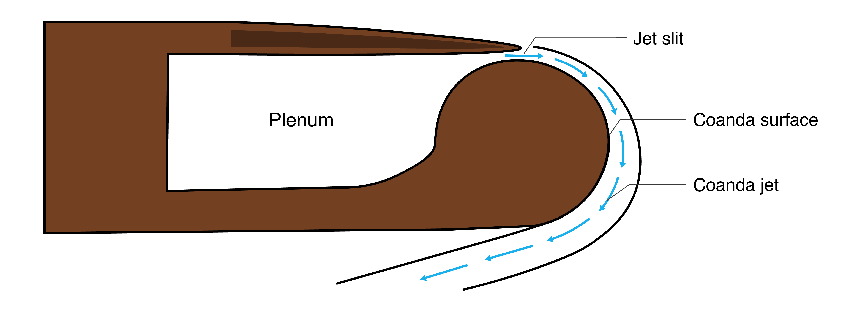
\includegraphics[width=10cm]{images/Theory-CFD/Coanda-effect.png}
    % \caption{Concept of Coanda effect: A fluid jet emerging from the orifice tends to adhere to the adjacent curved surface.}
    \caption{Demonstration of the Coanda effect: Visualization of a fluid jet adhering to and flowing along a curved surface, illustrating the fundamental principle utilized in the HOMER nozzle design.}
    \label{fig:Coanda}
  \end{figure}
% \section{Flow Simulation}
\section{Governing equations} \label{goveq}
In this section, we talk about the mathematical equations that govern the fluid flow in the nozzle setup. The computational domain for our fluid flow problem is shown in Figure \ref{fig:Domain}. We consider the same homogenous fluid for both primitive jets. This refers to streams with the same chemical and physical properties, i.e.; the density of the fluid \gls{rho} remains constant. The fluid in consideration is air in ideal gas conditions. The Navier Stokes Equations (NSE) can then be used to mathematically model the flow of an incompressible Newtonian fluid within the computational domain, given as, 
\begin{figure}[ht]
  \centering
  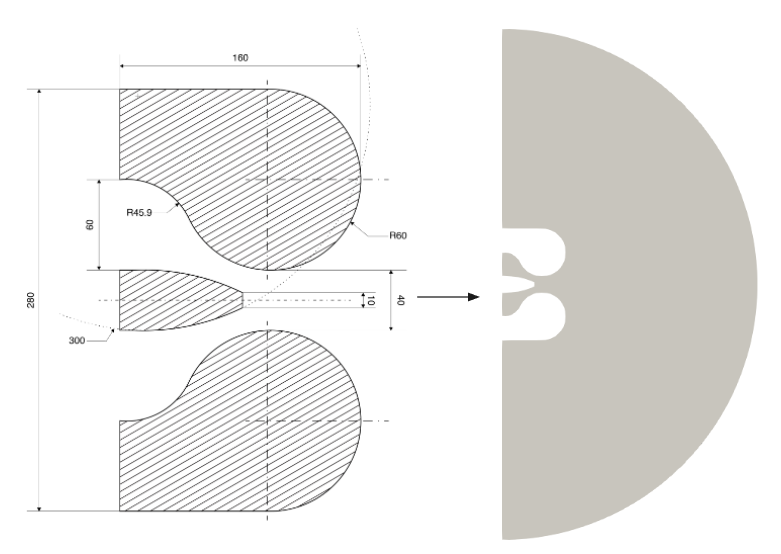
\includegraphics[width=12cm]{images/Theory-CFD/Flow Domain.png}
  \caption{Visualization of the HOMER Nozzle: Left - Geometry of the modified HOMER nozzle; Right - \glsentryshort{CAD} model showcasing the computational simulation domain.}
  \label{fig:Domain}
\end{figure}
\begin{equation}
  \begin{aligned}
  \frac{\partial u_i}{\partial x_i}&=0\\
  \frac{\partial u_i}{\partial t}+u_j \frac{\partial u_i}{\partial x_j}&=\frac{-1}{\rho} \frac{\partial p}{\partial x_i}+\nu \frac{\partial^2 u_i}{\partial x_j^2}
  \end{aligned}
  \end{equation}
where, \gls{ui} is the flow velocity in the spatial direction $x_i$, \gls{nu} is the kinematic viscosity, \gls{mu} is the dynamic viscosity ($\nu = \mu / \rho$), and \gls{p} is the pressure. We set constant velocities at the two inlets based on which a velocity profile corresponding to a fully-developed turbulent plane channel flow is computed at the inlet channels $\partial{\Omega_{in}}$. At the walls $\partial{\Omega_{wall}}$, we apply no-slip boundary conditions. We impose zero-gradient Neumann boundary conditions on the flow quantities at the outlet.\\
Turbulence, characterized by its unsteady, highly irregular, and energy-dissipative behaviors at high Reynolds numbers, causes minute fluctuations in velocity, pressure, and temperature across varying scales. While a DNS could theoretically capture these fluctuations by solving the NSE, the immense computational resources required render it impractical for most engineering simulations. 
% Turbulence modelling serves as a pragmatic approach to predict time-averaged fields without needing to resolve every turbulent detail.
Turbulence modelling using \gls{RANS} equations offers a practical compromise by solving time-averaged equations for steady-state or unsteady RANS (URANS) flows. RANS relies on turbulence models to account for unresolved turbulence effects, allowing for efficient simulations of complex engineering systems without resolving every turbulent detail. The underlying principle is to consider the flow as the sum of the mean flow and turbulent/fluctuating components. For a steady-state flow field, Reynolds decomposition is applied to flow quantities. For example, the flow velocity is expressed as $u_i = \bar{u}_i + u_i^{\prime}$, where $\bar{u}_i$ is the mean velocity and $u_i^{\prime}$ is the fluctuating turbulent component. The Reynolds averaging process introduces an additional term to the NSE known as Reynolds stress. By substituting the averaged quantities in the NSE, we obtain the RANS equations for our steady-state, 2D incompressible flow as,
\begin{equation}
  \begin{aligned}
  \frac{\partial \bar{u}_i}{\partial x_i}&=0 \\
  \rho \bar{u}_j \frac{\partial \bar{u}_i}{\partial x_j}&= - \frac{\partial \bar{p}}{\partial x_i} + \frac{\partial}{\partial x_j}     \left[ \mu \left(\frac{\partial \bar{u}_i}{\partial x_j}+\frac{\partial \bar{u}_j}{\partial x_i}\right) - \rho \overline{u_i^{\prime} u_j^{\prime}} \right] 
  \end{aligned}
\end{equation}
where, $- \rho \overline{u_i^{\prime} u_j^{\prime}}$ is the Reynolds stress tensor term and represents the effect of the small-scale turbulence on the average flow and $\bar{p}$ is the averaged pressure. The RANS equations have no unique solution because they are not in closed form, that is the unknowns are more than the equations. Thus, additional equations are needed for turbulence closure. The most common strategy used in CFD is to relate the Reynolds stress to the shear rate by the Boussinesq relationship:
% \begin{equation}
%   u_i^{\prime} u_j^{\prime}=2 \frac{\mu_t}{\rho} S_{i j} \quad \text { with } \quad S_{i j}=\frac{1}{2}\left(U_{i, j}+U_{j, i}\right)
% \end{equation}
\begin{equation}
\overline{u'_i u'_j} = - \nu_t \left( \frac{\partial \bar{u}_i}{\partial x_j} + \frac{\partial \bar{u}_j}{\partial x_i} \right) + \frac{2}{3} k \delta_{ij}
\end{equation}
where, \gls{k} is the turbulent kinetic energy and \gls{delta_ij} is the Kronecker delta, which is 1 if $i = j$ and 0 otherwise. \gls{nut} is the turbulent viscosity, computed from the turbulence models. Some of the RANS-based turbulence models are outlined below: 
\begin{enumerate}
  \item The Spalart-Allmaras model is a computationally efficient, one-equation model that solves for a single variable $\nu_t$.
  % This model is particularly suited for aerodynamic flows, offering reliable predictions with reduced computational cost.
  \item The $k-\epsilon$ model resolves turbulence through two equations: one for turbulent kinetic energy $k$ and another for the rate of dissipation of turbulent kinetic energy \gls{epsilon}. 
  % These equations govern the behavior of turbulence in a wide range of flows, from boundary layers to free shear flows.
  \item The $k-\omega$ model is another two-equation model that features transport equations for $k$ and a specific rate of turbulence dissipation \gls{omega}. This model is particularly advantageous in accurately predicting near-wall flows and is less susceptible to numerical issues than the $k-\epsilon$ model in adverse pressure gradient regions. 
  \item The $k-\omega$  \gls{SST} model combines aspects of the $k-\epsilon$ model near walls and the $k-\omega$ model away from walls to provide accurate predictions in both regions. The $k-\omega$ SST model is particularly suitable for boundary layer flows, capturing the near-wall behavior accurately while providing robust predictions in the outer flow regions. Its versatility and computational efficiency make it a popular choice for a wide range of engineering applications.
\end{enumerate}
For the purposes of this work, the $k-\omega$ SST turbulence model has been adopted.
\section{Numerical analysis}
Numerical analysis on PDEs - in our case, the RANS equations, is performed by discretizing the continuous domain into a discrete setup. This results in a system of algebraic equations, usually linear systems, that can be solved by iterative techniques such as Jacobi or Gauss-Seidel. Multigrid methods are another class of iterative numerical techniques used to solve discretized PDEs by employing a hierarchy of grids with varying levels of resolution - from coarse to fine - to accelerate convergence. \\
Some commonly used discretization techniques are the \gls{FDM}, \gls{FEM}, and \gls{FVM}. All three methods end up solving one (or several) system(s) of linear equations to compute an approximate numerical solution to the PDE at hand. And for all three methods, these linear systems are sparse, and the equation for an unknown $u_i$ involves a few neighbors of point $i$. Overall, FDM is mostly used for geometries that can be discretized by structured grids (e.g., rectangles), while FEM and FVM are more suitable for complex domains. \\
FVM discretizes PDEs by dividing the computational domain into finite volumes or cells. It conservatively approximates integral forms of conservation laws within each cell. The method calculates fluxes across cell interfaces, preserving conservation principles, making it particularly suited for problems involving fluid flow, heat transfer, and other conservation phenomena. As FVM is based on the integral formulation of a conservation law, it is mainly used to solve PDEs in fluid dynamics, which involve fluxes of the conserved variable. In this thesis, we are only interested in the discretization of PDEs using FVM, which is the most widely used discretization approach in CFD solvers. 
% In the case of non-linear systems arising from discretization, linearization schemes are required to convert the non-linearity into a sequence of linear systems: a sequence of linearized equations is solved iteratively, converging to the solution of the non-linear system. 
\section{Simulation setup} \label{setup}
Trancossi and Dumas \cite{trandum} proposed a mathematical model of the HOMER nozzle and carried out 2D, incompressible flow simulations on this geometry. The simplified model predicts the detachment angle of the jet stream over the curved surface. The nozzle chosen for our study is a slightly modified version of a thrust-vectoring propulsive HOMER nozzle. The modified design is inspired by the numerical investigation and experimental validation of Kara and Erpulat \cite{kara}. The geometry adopted for the simulations as well as the computational domain are depicted in Figure \ref{fig:Domain}. The selected channel length ensures the mean flow quantities are fully developed, hence establishing steady-state conditions. The meshing and simulation are carried out on \verb|OpenFOAM| which uses finite volume methods to discretize the PDEs. 
\subsection{Mesh generation}
The geometry is created using FreeCAD \cite{FreeCAD} and patch names are assigned based on the type of boundaries.  The meshing process on \verb|OpenFOAM| begins with the discretization of the geometry into hexahedral blocks using \verb|blockMesh|. Then, \verb|snappyHexMesh| refines the mesh based on parameters specified in \verb|snappyHexMeshDict|. This includes defining refinement controls, snapping settings, adding boundary layers, and ensuring mesh quality. The process iteratively refines the mesh until the desired quality and resolution are achieved, enabling accurate simulations of the geometry's physical behavior. An unstructured, 3D hybrid mesh with tetrahedral and hexahedral elements has been generated for the computational domain and is enhanced by boundary layer refinement and a refinement box around the nozzle region.
\subsection{Boundary conditions and solver settings}
% An incompressible steady-state CFD simulation is carried out on the mesh by setting appropriate boundary and initial conditions. For $k$, \( \omega \) and turbulent viscosity $\nu_t$, low Reynolds number wall functions are applied at walls to account for near-wall turbulence effects. This ensures accurate modeling of turbulence near boundaries. Pressure is set to zero gradient at the walls to maintain a neutral pressure condition. Adiabatic stationary walls with no slip conditions are prescribed at the Coanda surfaces as well as the inner walls of the nozzle. Inlets are prescribed with fixed values of velocities to define the flow entering the domain. Both the inlet turbulence intensities are set to 1\% (medium turbulence). Additionally, a pressure outlet boundary condition is used to specify the pressure at outlets, allowing flow to exit the domain without reflecting back. These boundary conditions collectively ensure proper representation of the flow behavior within the computational domain. The simulations are performed using the \verb|simpleFoam| solver which utilizes the SIMPLE (Semi-Implicit Method for Pressure Linked Equations) algorithm for pressure-velocity coupling. This method iteratively resolves the momentum and pressure equations until a predetermined convergence criterion is satisfied. The $k-\omega$ \gls{SST} turbulence model is utilized, and the kinematic viscosity of the fluid is taken as $1.51e^{-5}$. The convective term of velocity is discretized using the linear UpwindV scheme whereas the divergence term of velocity is discretized using a bounded Gauss linear scheme. For the discretization of the divergence of the turbulence fields $k$, $\omega$, $\nu_t$, a bounded Gauss upwind scheme is used. In this case, the convergence criterion was set to $10e^{-6}$ for the pressure field and $10e^{-8}$ for all other quantities. 
We carry out an incompressible steady-state CFD simulation on the mesh, setting appropriate boundary and initial conditions. By applying low Reynolds number wall functions for $k$, $\omega$, and turbulent viscosity $\nu_t$ at walls, we account for near-wall turbulence effects, ensuring accurate modelling near boundaries. We also prescribe adiabatic stationary walls with no slip conditions, and pressure to zero gradient, at the Coanda surfaces and the inner walls of the nozzle. We define the flow entering the domain by prescribing inlets with fixed velocities and set both inlet turbulence intensities to 1\% (medium turbulence). Furthermore, we specify the pressure at outlets through a pressure outlet boundary condition, allowing flow to exit the domain without reflecting back. These actions collectively ensure the proper representation of flow behavior within the computational domain. The \verb|simpleFoam| solver is the tool we use for the simulations, employing the \gls{SIMPLE} algorithm for effective pressure-velocity coupling. We iteratively resolve the momentum and pressure equations until achieving a predetermined convergence criterion. The $k-\omega$ SST turbulence model serves our purposes, with the fluid's kinematic viscosity set at $1.51 \times {10}^{-5}$. For velocity's convective term, we use the linear Upwind scheme for discretization, while the divergence term undergoes discretization via a bounded Gauss linear scheme. For the turbulence fields $k$, $\omega$, $\nu_t$, we employ a bounded Gauss upwind scheme for discretization. We have set the convergence criterion to ${10}^{-6}$ for the pressure field and ${10}^{-8}$ for all other quantities.
\section{Simulation results}
In this section, we highlight the simulation results of a few flow scenarios. Figure \ref{vel} showcases the velocity fields of four distinct cases and their behavior towards the Coanda surfaces. Figure \ref{pres} presents the pressure fields for the same cases. 
\begin{figure}[ht]
  \centering
  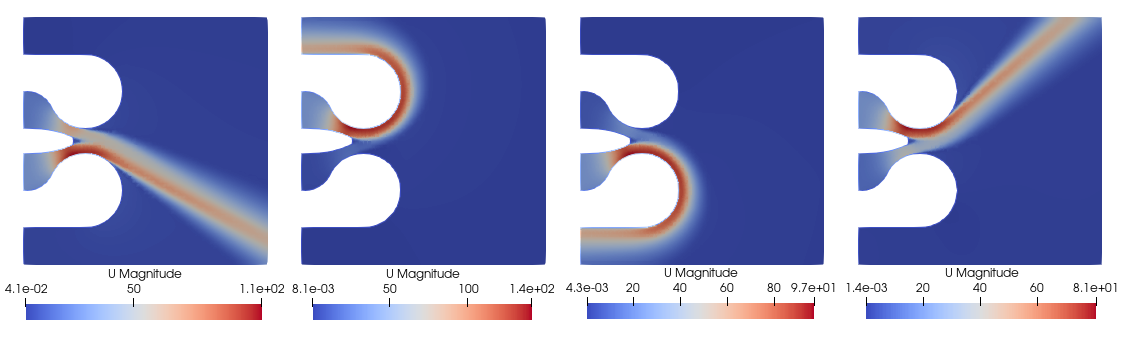
\includegraphics[width=15.5cm]{images/Theory-CFD/cfdvel.png}
  \caption{Velocity fields from four simulation cases, from left to right: (a) (18 m/s, 27 m/s) shows jet deflection towards the bottom surface, (b) (35 m/s, 5 m/s) shows Coanda adhesion to the top surface, (c) (6 m/s, 24 m/s) shows Coanda adhesion to the bottom surface, (d) (20 m/s, 10 m/s) shows jet deflection towards the top surface, where (Inlet 1, Inlet 2) describe the initial velocities.}
  \label{vel}
\end{figure}
\begin{figure}[ht]
  \centering
  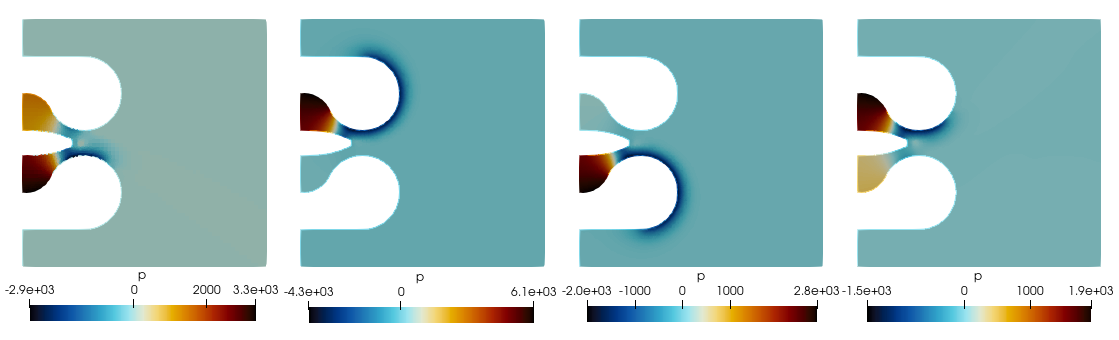
\includegraphics[width=15.5cm]{images/Theory-CFD/cfdp.png}
  \caption{Results from simulations showcasing pressure fields for four cases of interest, from left to right: (a) (18 m/s, 27 m/s), (b) (35 m/s, 5 m/s), (c) (6 m/s, 24 m/s), and (d) (20 m/s, 10 m/s). The initial velocities are enclosed as (Inlet 1, Inlet 2).}
  \label{pres}
\end{figure}